\section{Preparation of Distributions}

We investigate, how the above circuit encoding schemes can be applied in the preparation of states, which computational basis measurements are samples from specific distributions.

\subsection{Generic Q-samples}

In general, we define Q-samples to be quantum states, which measured in the computational basis reproduce a given probability distribution.

\begin{definition}[Q-sample]
    Given a probability distribution $\probtensor:\atomstates\rightarrow\rr$ (i.e. $\contraction{\probtensor}=1$ and $\zeros \prec \probtensor$) its q-sample is
    \begin{align*}
        \qstateofat{\probtensor}{\shortcatvariables}
        = \sum_{\shortcatindicesin} \sqrt{\probat{\indexedshortcatvariables}} \cdot \onehotmapofat{\shortcatindices}{\shortcatvariables} \, .
    \end{align*}
\end{definition}

%% Low Paper
In \cite{low_quantum_2014} the Q-sample has been introduced.
It prepares a scheme to realize property 1 (purity) + 2 (q-sampling) of a qpdf, but fails to realize property 3 (q-stochasticity).
The q-sample can be prepared for Bayesian Networks, where each child qubit is prepared densely by C-NOTs conditioning on parent qubits.

Q-samples can be prepared by \activationCircuit{}s acting on uniform quantum states (Hadamard gates acting on ground state).

%    \begin{lemma}
%        The \activationCircuit{} of $\probwith$ acting on the uniform state of $\shortcatvariables$ prepares a q-sample.
%    \end{lemma}
%    \begin{proof}
%        Follows directly from construction:
%        The uniform state is the action of Hadamard gates on the ground state $\onehotmapofat{0}{\shortcatvariables}$, which prepares the state $\normalizationof{\ones}{\shortcatvariables}$.
%        The diagonal \activationCircuit{} transforms
%    \end{proof}

Doing rejection sampling on the ancilla qubit corresponds with sampling from the normalized contraction with the activation tensor.

\begin{lemma}
    Given a distribution $\probat{\shortcatvariables}$, we construct a circuit preparing its q-sample and add the ancilla encoding of a tensor $\hypercoreat{\shortcatvariables}$.
    The rejection sampling scheme, measuring the ancilla qubit and the $\shortcatvariables$ qubits, rejecting the ancilla qubit measured as $0$, prepares samples from the distribution
    \begin{align*}
        \normalizationof{\probat{\shortcatvariables},\hypercoreat{\shortcatvariables}}{\shortcatvariables} \, .
    \end{align*}
\end{lemma}

\subsection{Ancilla Augmentation}

%% NEEDED ALREADY HERE?
For more flexible sampling schemes of \ComputationActivationNetworks{} we need to introduce ancilla qubits.

\begin{definition}[Ancilla Augmented Distribution]
    Let $\probwith$ be a probability distribution over variables $\shortcatvariables$.
    Another joint distribution $\secprobtensor$ of $\shortcatvariables$ and ancilla variables $\avariables$ is called an ancilla augmented distribution, if
    \begin{align*}
        \secprobat{\shortcatvariables|\avariables=\onesat{[\seldim]}} = \probwith \, .
    \end{align*}
\end{definition}

Sampling from the distribution can be done by rejection sampling on the ancilla augmented distribution, measuring all variables and rejecting all samples where an ancilla variable is $0$.

%% Usage through rejection sampling
Given an augmented Q-sample of a distribution, we can prepare samples from the distribution by rejection sampling, measuring all variables $\shortcatvariables$ and $\avariables$ and rejecting all samples where an ancilla qubit is measured as $0$.

%% Usage as forward inferer
When sampling from probability distributions, we can use these samples to estimate probabilistic queries.
Building on such particle-based inference schemes, we can perform various inference schemes for \ComputationActivationNetworks{}, such as backward inference and message passing schemes.

%% Main point: Construction by activation circuits
Given a distribution $\probat{\shortcatvariables}$ we add an ancilla variable $\avariable$ and define the augmented distribution (see \figref{fig:ancillaAugmentation})
\begin{align*}
    \secprobat{\avariable,\shortcatvariables} =
    \frac{1}{\prod_{\catenumeratorin}\catdimof{\catenumerator}}
    \sum_{\shortcatindicesin} \onehotmapofat{\shortcatindices}{\shortcatvariables}
    \otimes \Big(
    \probat{\shortcatindices} \cdot \tbasisat{\avariable} + (1- \probat{\shortcatindices}) \cdot \fbasisat{\avariable}
    \Big) \, .
\end{align*}
Then we have
\begin{align*}
    \secprobat{\shortcatvariables|\avariable=1} = \probat{\shortcatvariables} \, .
\end{align*}

\begin{figure}
    \begin{center}
        \begin{tikzpicture}[scale=0.35,thick] % , baseline = -3.5pt

    \node[anchor=center] (text) at (28,1) {${b)}$};

    \begin{scope}
        [shift={(31,-7)}]

        \node[anchor=center] (text) at (-1,6.5) {$\avariableof{\insymbol}$};
        \node[anchor=center] (text) at (12,6.5) {$\avariableof{\outsymbol}$};

        \draw (5.5,1) -- (5.5,5.5);
        \drawvariabledot{5.5}{4}
        \drawvariabledot{5.5}{1}

        \draw (1,6.5) -- (2,6.5);
        \draw (2,5.5) rectangle (9,7.5);
        \node[anchor=center] (text) at (5.65,6.5) {$\qcbencodingof{\probtensor}$};
        \draw (9,6.5) -- (10,6.5);

        \draw[dashed] (0.5,5) -- (10.5,5);

        \draw (1,4) -- (10,4);

        \node[anchor=center] (text) at (3,2.75) {$\vdots$};
        \node[anchor=center] (text) at (-1,2.5) {$\catvariableof{[\atomorder],\insymbol}$};

        \node[anchor=center] (text) at (8,2.75) {$\vdots$};
        \node[anchor=center] (text) at (12,2.5) {$\catvariableof{[\atomorder],\outsymbol}$};

        \draw (1,1) -- (10,1);

    \end{scope}


    \node[anchor=center] (text) at (1,1) {${a)}$};

    \draw[->-] (4.5,-1) -- (4.5,1) node[midway, right]{$\avariable$};
    \draw (3,-1) rectangle (6,-4);
    \node[anchor=center] (text) at (4.5,-2.5) { $\secprobtensor$};

    \draw[->-] (3.5,-6) -- (3.5,-4);
    \node[anchor=center] (text) at (4.5,-4.75) {$\cdots$};
    \node[anchor=center] (text) at (4.5,-6) {$\shortcatvariables$};
    \draw[->-] (5.5,-6) -- (5.5,-4);

    \node[anchor=center] (text) at (8,-2.5) {${=}$};

    \begin{scope}
        [shift={(3,2)}]

        \node[anchor=center] (text) at (8,-4.5) {$\sum_{\shortcatindices}$};

        \draw[->-] (15,-1) -- (15,1) node[midway, right]{$\avariable$};
        \draw (10,-4) rectangle (20,-1);
        \node[anchor=center] (text) at (15,-2.5) {$\begin{bmatrix}
                                                       1 - \probat{\indexedshortcatvariables} \\
                                                       \probat{\indexedshortcatvariables}
        \end{bmatrix}$};

        \draw (13,-5) rectangle (17,-7);
        \node[anchor=center] (text) at (15,-6) {$\onehotmapof{\shortcatindices}$};
        \draw[->-] (13.5,-7) -- (13.5,-9);
        \node[anchor=center] (text) at (15,-7.4) {$\cdots$};
        \node[anchor=center] (text) at (15,-8.5) {$\shortcatvariables$};
        \draw[->-] (16.5,-7) -- (16.5,-9);

    \end{scope}

\end{tikzpicture}
    \end{center}
    \caption{
        Ancilla augmentation of a distribution $\probwith$.
        a) Augmented distribution $\secprobat{\avariable,\shortcatvariables}$ with the property that $\probwith = \secprobat{\shortcatvariables|\avariable=1}$.
        b) Preparation of the augmented distribution by the \activationCircuit{} of $\probwith$.
    }\label{fig:ancillaAugmentation}
\end{figure}

\subsection{Amplitude Amplification}

Note, that the variable qubits are uniformly distributed when only the computation circuit is applied.
When sampling the probability distribution, we need the aniclla qubits to be in state $1$ in order for the sample to be valid.
Any other states will have to be rejected.

Classically, this can be simulated in the same way:
Just draw the variables from uniform, calculate the value qubit by a logical circuit inference and accept with probability by the computed value.

For this procedure to be more effective (and in particular not having an efficient classical pendant), we need amplitude amplification on the value qubit.
This can provide a square root speedup in the complexity compared with classical rejection sampling.

\textbf{Open Question:} Is there a way to avoid amplitude amplification and use a more direct circuit implementation of the activation network?
- Cannot be the case, when the encoding is determined by the activation tensor alone: Needs to use the computated statistic as well.

\subsection{Sampling from \ComputationActivationNetworks{} as Quantum Circuits}

\red{So far: Sample from \HybridLogicNetworks{}, would need qudits for for more general \ComputationActivationNetworks{}.}

\tnreason{} provides tensor network representations of knowledge bases and exponential families following a Computation Activation architecture.
Here are some ideas to utilize quantum circuits for sampling from \ComputationActivationNetworks{}.
We can produce Q-samples for ancilla augmented \ComputationActivationNetworks{}  using \computationCircuits{} and \activationCircuits{}:
\begin{itemize}
    \item For each (sub-) statistic, prepare a qubit by \ComputationCircuits{}
    \item Based on the computed qubits, prepare ancilla qubits by \ActivationCircuits{} to the activation cores.
\end{itemize}

\begin{figure}
    \begin{center}
        \usetikzlibrary{decorations.pathreplacing,shapes.geometric,calc}


\begin{tikzpicture}[scale=0.35, thick] % , baseline = -3.5pt

    %% Ancilla Qubits

    \draw (-1,16) rectangle (1,18);
    \node[anchor=center] (text) at (0,17) {$\onehotmapof{0}$};
    \draw (1,17) -- (13.5,17);
    \draw (13.5,16) rectangle (16.5,18);
    \node[anchor=center] (text) at (15,17) {$\qcaencodingof{\hypercoreof{\seldim-1}}$};
    \draw (16.5,17) -- (20,17);

    \draw (15,10) -- (15,16);
    \drawvariabledot{15}{10}

    \node[rotate=45] at (13.5,15) {$\cdots$};
    \node[rotate=45] at (13.5,8) {$\cdots$};

    \node[anchor=center] (text) at (0,15.25) {$\vdots$};
    \node[anchor=east] (text) at (-2,15) {Ancilla Qubits};%{$\avariableof{[\seldim]}$};

    \draw (-1,12) rectangle (1,14);
    \node[anchor=center] (text) at (0,13) {$\onehotmapof{0}$};
    \draw (1,13) -- (11,13);
    \draw (11,12) rectangle (13,14);
    \node[anchor=center] (text) at (12,13) {$\qcaencodingof{\hypercoreof{0}}$};
    \draw (13,13) -- (20,13);

    \draw (12,6) -- (12,12);
    \drawvariabledot{12}{6}

    %% Statistic Qubits
    \draw[dashed] (-3,11.5) -- (22.5,11.5);

    \draw (-1,9) rectangle (1,11);
    \node[anchor=center] (text) at (0,10) {$\onehotmapof{0}$};
    \draw (1,10) -- (7.5,10);
    \draw (7.5,9) rectangle (10.5,11);
    \node[anchor=center] (text) at (9,10) {$\qcbencodingof{f_{\seldim-1}}$};
    \draw (10.5,10) -- (20,10);

    \draw (8.5,3) -- (8.5,9);
    \drawvariabledot{8.5}{3}
    \draw (9.5,-1) -- (9.5,9);
    \drawvariabledot{9.5}{-1}

    \node[rotate=45] at (7.5,8) {$\cdots$};
    \node[rotate=45] at (7.5,1) {$\cdots$};

    \node[anchor=center] (text) at (0,8.25) {$\vdots$};
    \node[anchor=east] (text) at (-2,8) {Statistic Qubits};%{$\headvariables$};

    \draw (-1,5) rectangle (1,7);
    \node[anchor=center] (text) at (0,6) {$\onehotmapof{0}$};
    \draw (1,6) -- (5,6);
    \draw (5,5) rectangle (7,7);
    \node[anchor=center] (text) at (6,6) {$\qcbencodingof{f_{0}}$};
    \draw (7,6) -- (20,6);

    \draw (5.5,3) -- (5.5,5);
    \drawvariabledot{5.5}{3}
    \draw (6.5,-1) -- (6.5,5);
    \drawvariabledot{6.5}{-1}

    %% Distributed Qubits
    \draw[dashed] (-3,4.5) -- (22.5,4.5);

    \draw (-1,2) rectangle (1,4);
    \node[anchor=center] (text) at (0,3) {$\onehotmapof{0}$};
    \draw (1,3) -- (2,3);
    \draw (2,2) rectangle (4,4);
    \node[anchor=center] (text) at (3,3) {$H$};

    \draw (4,3) -- (20,3);

    \node[anchor=center] (text) at (0,1.25) {$\vdots$};
    \node[anchor=east] (text) at (-2,1) {Distributed Qubits};%{$\shortcatvariables$};

    \draw (-1,-2) rectangle (1,0);
    \node[anchor=center] (text) at (0,-1) {$\onehotmapof{0}$};
    \draw (1,-1) -- (2,-1);
    \draw (2,-2) rectangle (4,0);
    \node[anchor=center] (text) at (3,-1) {$H$};

    \draw (4,-1) -- (20,-1);

    \drawqcmeasuresymbol{21}{17}
    \node[anchor=center] (text) at (21,15.25) {$\vdots$};
    \drawqcmeasuresymbol{21}{13}

    \drawqcmeasuresymbol{21}{3}
    \node[anchor=center] (text) at (21,1.25) {$\vdots$};
    \drawqcmeasuresymbol{21}{-1}

\end{tikzpicture}
    \end{center}
    \caption{
        Quantum Circuit to reproduce a \ComputationActivationNetwork{} (with elementary activation) by rejection sampling.
        We measure the distributed qubits $\shortcatvariables$ and the ancilla qubits $\avariableof{[\seldim]}$ and reject all samples, where an ancilla qubit is measured as $0$.
    }\label{fig:caCircuit}
\end{figure}


\section{Implementation}

The introduced quantum circuit preparation schemes have been implemented in the python package \qcreason{}, which consists in three layers:
\begin{center}
    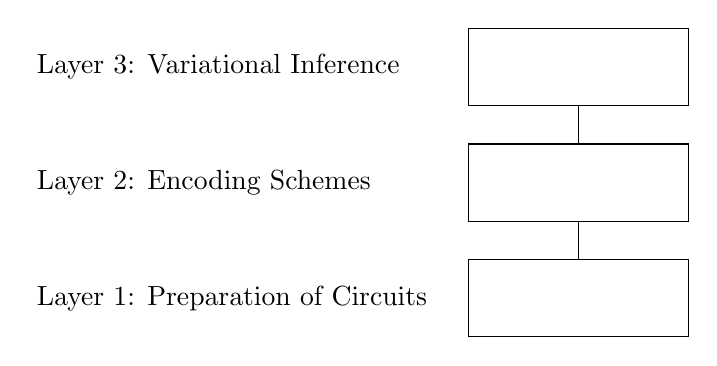
\begin{tikzpicture}[scale=0.35,yscale=0.7]
    \draw (-10,10) rectangle (-2,14);
    \node [anchor=center] at (-6,12) {\spreasoning{}};
    \node [anchor=west] at (-26,12) {Layer 3: Variational Inference};

    \draw (-6,10) -- (-6,8);
    \draw (-10,4) rectangle (-2,8);
    \node [anchor=center] at (-6,6) {\sprepresentation{}};
    \node [anchor=west] at (-26,6) {Layer 2: Encoding Schemes};

    \draw (-6,4) -- (-6,2);
    \draw (-10,-2) rectangle (-2,2);
    \node [anchor=center] at (-6,0) {\spengine{}};
    \node [anchor=west] at (-26,0) {Layer 1: Preparation of Circuits};
\end{tikzpicture}
\end{center}